\documentclass{standalone}
\usepackage{tikz}
\usetikzlibrary{patterns, positioning}


\begin{document}
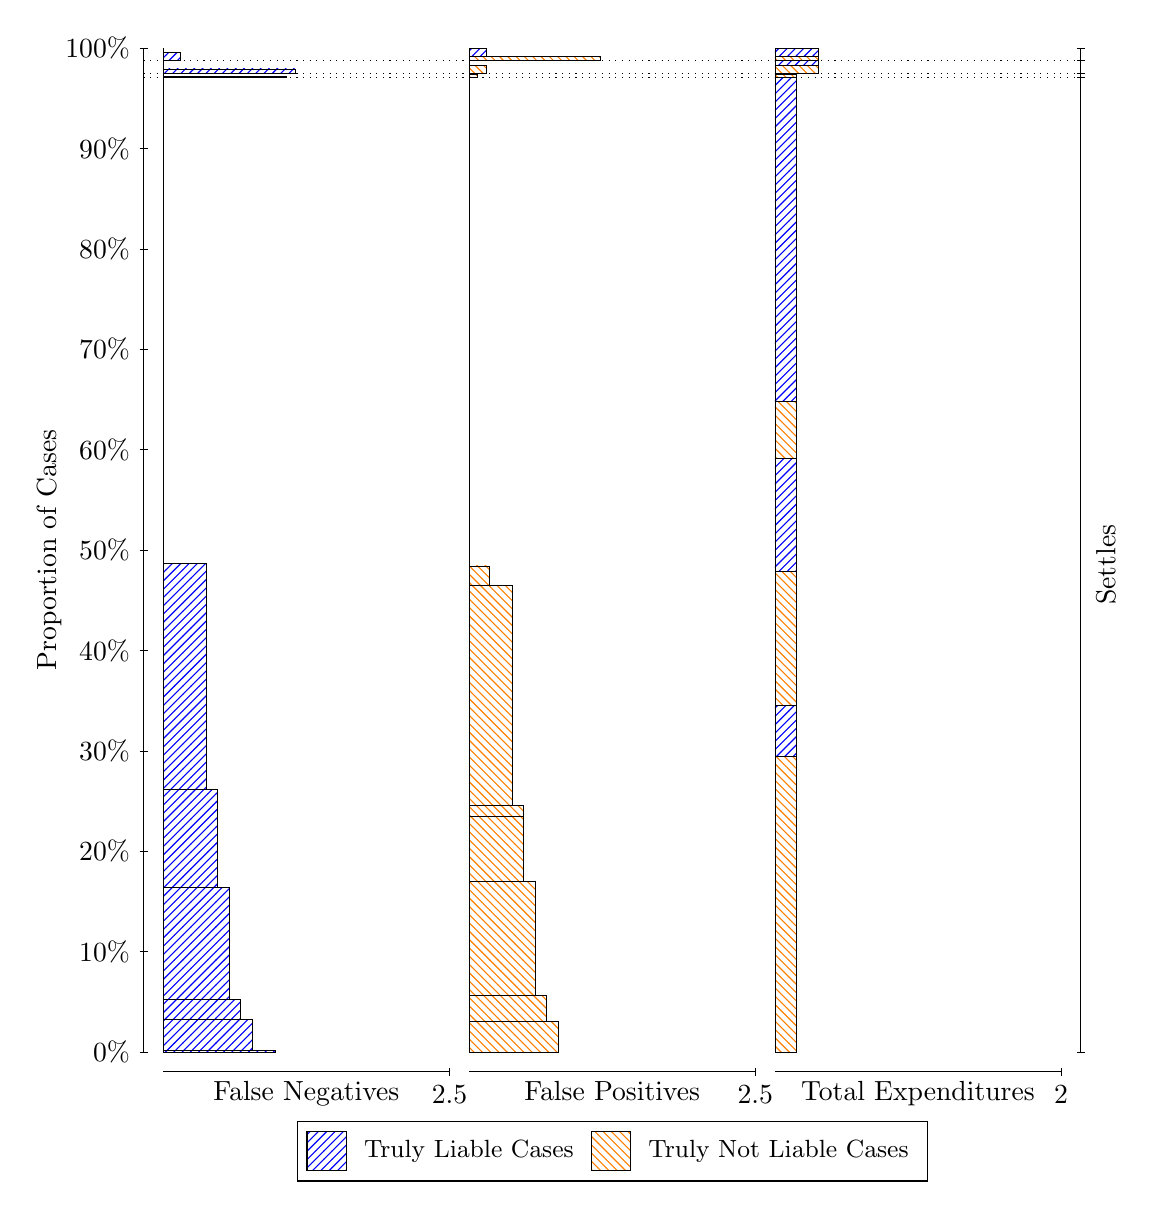
\begin{tikzpicture}
\draw[black, very thin] (1.5,1.75) -- (1.5,14.5);
\node[rotate=90, text=black, anchor=center] at (0.3, 8.125) {Proportion of Cases};
\draw[black, very thin] (1.45,1.75) -- (1.55,1.75);
\node[text=black, anchor=east] at (1.45, 1.75) {0\%};
\draw[black, very thin] (1.45,3.025) -- (1.55,3.025);
\node[text=black, anchor=east] at (1.45, 3.025) {10\%};
\draw[black, very thin] (1.45,4.3) -- (1.55,4.3);
\node[text=black, anchor=east] at (1.45, 4.3) {20\%};
\draw[black, very thin] (1.45,5.575) -- (1.55,5.575);
\node[text=black, anchor=east] at (1.45, 5.575) {30\%};
\draw[black, very thin] (1.45,6.85) -- (1.55,6.85);
\node[text=black, anchor=east] at (1.45, 6.85) {40\%};
\draw[black, very thin] (1.45,8.125) -- (1.55,8.125);
\node[text=black, anchor=east] at (1.45, 8.125) {50\%};
\draw[black, very thin] (1.45,9.4) -- (1.55,9.4);
\node[text=black, anchor=east] at (1.45, 9.4) {60\%};
\draw[black, very thin] (1.45,10.675) -- (1.55,10.675);
\node[text=black, anchor=east] at (1.45, 10.675) {70\%};
\draw[black, very thin] (1.45,11.95) -- (1.55,11.95);
\node[text=black, anchor=east] at (1.45, 11.95) {80\%};
\draw[black, very thin] (1.45,13.225) -- (1.55,13.225);
\node[text=black, anchor=east] at (1.45, 13.225) {90\%};
\draw[black, very thin] (1.45,14.5) -- (1.55,14.5);
\node[text=black, anchor=east] at (1.45, 14.5) {100\%};

\draw[black, very thin] (13.4,1.75) -- (13.4,14.5);
\draw[black, very thin] (13.35,1.75) -- (13.45,1.75);
\node[anchor=west] at (13.35, 1.75) {};
\draw[black, very thin] (13.35,14.127) -- (13.45,14.127);
\node[anchor=west] at (13.35, 14.127) {};
\draw[black, very thin] (13.35,14.178) -- (13.45,14.178);
\node[anchor=west] at (13.35, 14.178) {};
\draw[black, very thin] (13.35,14.339) -- (13.45,14.339);
\node[anchor=west] at (13.35, 14.339) {};
\draw[black, very thin] (13.35,14.5) -- (13.45,14.5);
\node[anchor=west] at (13.35, 14.5) {};

\draw[black, very thin, pattern color=blue, pattern=north east lines] (1.75,1.75) rectangle (3.167,1.7714);
\draw[black, very thin, pattern color=blue, pattern=north east lines] (1.75,1.7714) rectangle (2.8763,2.1686);
\draw[black, very thin, pattern color=blue, pattern=north east lines] (1.75,2.1686) rectangle (2.731,2.4194);
\draw[black, very thin, pattern color=blue, pattern=north east lines] (1.75,2.4194) rectangle (2.5857,3.839);
\draw[black, very thin, pattern color=blue, pattern=north east lines] (1.75,3.839) rectangle (2.4403,5.084);
\draw[black, very thin, pattern color=blue, pattern=north east lines] (1.75,5.084) rectangle (2.295,7.9553);
\draw[black, very thin, pattern color=orange, pattern=north west lines] (1.75,7.9553) rectangle (1.75,14.127);
\draw[black, very thin, pattern color=blue, pattern=north east lines] (1.75,14.127) rectangle (3.3123,14.136);
\draw[black, very thin, pattern color=orange, pattern=north west lines] (1.75,14.136) rectangle (1.75,14.178);
\draw[black, very thin, pattern color=blue, pattern=north east lines] (1.75,14.178) rectangle (3.4213,14.234);
\draw[black, very thin, pattern color=orange, pattern=north west lines] (1.75,14.234) rectangle (1.75,14.339);
\draw[black, very thin, pattern color=blue, pattern=north east lines] (1.75,14.339) rectangle (1.968,14.445);
\draw[black, very thin, pattern color=orange, pattern=north west lines] (1.75,14.445) rectangle (1.75,14.5);
\draw[black, very thin, pattern color=orange, pattern=north west lines] (5.6333,1.75) rectangle (6.7597,2.1433);
\draw[black, very thin, pattern color=orange, pattern=north west lines] (5.6333,2.1433) rectangle (6.6143,2.4698);
\draw[black, very thin, pattern color=orange, pattern=north west lines] (5.6333,2.4698) rectangle (6.469,3.9212);
\draw[black, very thin, pattern color=orange, pattern=north west lines] (5.6333,3.9212) rectangle (6.3237,4.7427);
\draw[black, very thin, pattern color=orange, pattern=north west lines] (5.6333,4.7427) rectangle (6.3237,4.8772);
\draw[black, very thin, pattern color=orange, pattern=north west lines] (5.6333,4.8772) rectangle (6.1783,7.6714);
\draw[black, very thin, pattern color=orange, pattern=north west lines] (5.6333,7.6714) rectangle (5.8877,7.9221);
\draw[black, very thin, pattern color=blue, pattern=north east lines] (5.6333,7.9221) rectangle (5.6333,14.127);
\draw[black, very thin, pattern color=orange, pattern=north west lines] (5.6333,14.127) rectangle (5.7423,14.17);
\draw[black, very thin, pattern color=blue, pattern=north east lines] (5.6333,14.17) rectangle (5.6333,14.178);
\draw[black, very thin, pattern color=orange, pattern=north west lines] (5.6333,14.178) rectangle (5.8513,14.284);
\draw[black, very thin, pattern color=blue, pattern=north east lines] (5.6333,14.284) rectangle (5.6333,14.339);
\draw[black, very thin, pattern color=orange, pattern=north west lines] (5.6333,14.339) rectangle (7.3047,14.394);
\draw[black, very thin, pattern color=blue, pattern=north east lines] (5.6333,14.394) rectangle (5.8513,14.5);
\draw[black, very thin, pattern color=orange, pattern=north west lines] (9.5167,1.75) rectangle (9.7892,5.5003);
\draw[black, very thin, pattern color=blue, pattern=north east lines] (9.5167,5.5003) rectangle (9.7892,6.1483);
\draw[black, very thin, pattern color=orange, pattern=north west lines] (9.5167,6.1483) rectangle (9.7892,7.8503);
\draw[black, very thin, pattern color=blue, pattern=north east lines] (9.5167,7.8503) rectangle (9.7892,9.2913);
\draw[black, very thin, pattern color=orange, pattern=north west lines] (9.5167,9.2913) rectangle (9.7892,10.011);
\draw[black, very thin, pattern color=blue, pattern=north east lines] (9.5167,10.011) rectangle (9.7892,14.127);
\draw[black, very thin, pattern color=orange, pattern=north west lines] (9.5167,14.127) rectangle (9.7892,14.17);
\draw[black, very thin, pattern color=blue, pattern=north east lines] (9.5167,14.17) rectangle (9.7892,14.178);
\draw[black, very thin, pattern color=orange, pattern=north west lines] (9.5167,14.178) rectangle (10.062,14.284);
\draw[black, very thin, pattern color=blue, pattern=north east lines] (9.5167,14.284) rectangle (10.062,14.339);
\draw[black, very thin, pattern color=orange, pattern=north west lines] (9.5167,14.339) rectangle (10.062,14.394);
\draw[black, very thin, pattern color=blue, pattern=north east lines] (9.5167,14.394) rectangle (10.062,14.5);
\draw[black, dotted] (1.5,14.127) -- (13.4,14.127);
\draw[black, dotted] (1.5,14.178) -- (13.4,14.178);
\draw[black, dotted] (1.5,14.339) -- (13.4,14.339);
\draw[black, very thin] (1.75,1.5) -- (5.3833,1.5);
\node[text=black, anchor=north] at (3.5667, 1.5) {False Negatives};
\draw[black, very thin] (5.3833,1.45) -- (5.3833,1.55);
\node[text=black, anchor=north] at (5.3833, 1.45) {2.5};

\draw[black, very thin] (5.6333,1.5) -- (9.2667,1.5);
\node[text=black, anchor=north] at (7.45, 1.5) {False Positives};
\draw[black, very thin] (9.2667,1.45) -- (9.2667,1.55);
\node[text=black, anchor=north] at (9.2667, 1.45) {2.5};

\draw[black, very thin] (9.5167,1.5) -- (13.15,1.5);
\node[text=black, anchor=north] at (11.333, 1.5) {Total Expenditures};
\draw[black, very thin] (13.15,1.45) -- (13.15,1.55);
\node[text=black, anchor=north] at (13.15, 1.45) {2};

\node[text=black, centered, rotate=90] at (13.72, 7.9387) {Settles};




\draw (7.449999999999999,1.5) node[draw=none] (baseCoordinate) {};
\begin{scope}[align=center]
        \matrix[scale=0.5, draw=black, below=0.5cm of baseCoordinate, nodes={draw}, column sep=0.1cm]{
            \node[rectangle, draw, minimum width=0.5cm, minimum height=0.5cm, pattern color=blue, pattern=north east lines] {}; &
            \node[draw=none, font=\small, text=black] (B) {Truly Liable Cases}; &
            \node[rectangle, draw, minimum width=0.5cm, minimum height=0.5cm, pattern color=orange, pattern=north west lines] {}; &
            \node[draw=none, font=\small, text=black] (B) {Truly Not Liable Cases}; \\
            };
\end{scope}

\end{tikzpicture}
\end{document}